\mysubsubsection{Stereo}

We performed our experiments on the Book sequence from Middlebury stereo
datasets.~\cite{middlebury_stereo}. We use 7 images with the
resolution of $695\times555$ and optimize for 256 disparity labels. We
recoreded both single thread energy and system energy (minimum energy
so far from all threads) against time. Since the order of labels to be
expanded or fused will have impact on minimization, we randomly
shuffled 256 labels and provide this order to all methods.

\begin{figure}[tb]
  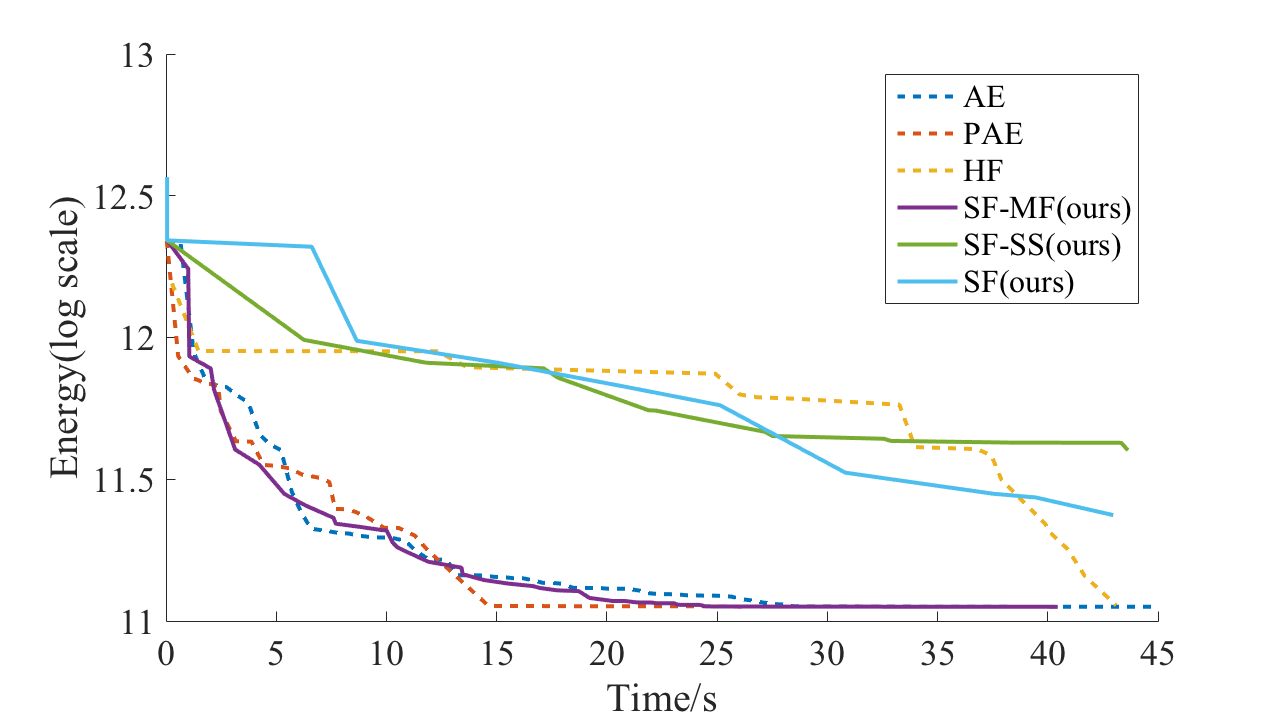
\includegraphics[width=\columnwidth]{figure/stereo_global.png}
  \caption{The energy minimization process of difference parallel systems.}
  \label{fig:stereo_global}
\end{figure}

\begin{figure}[tb]
  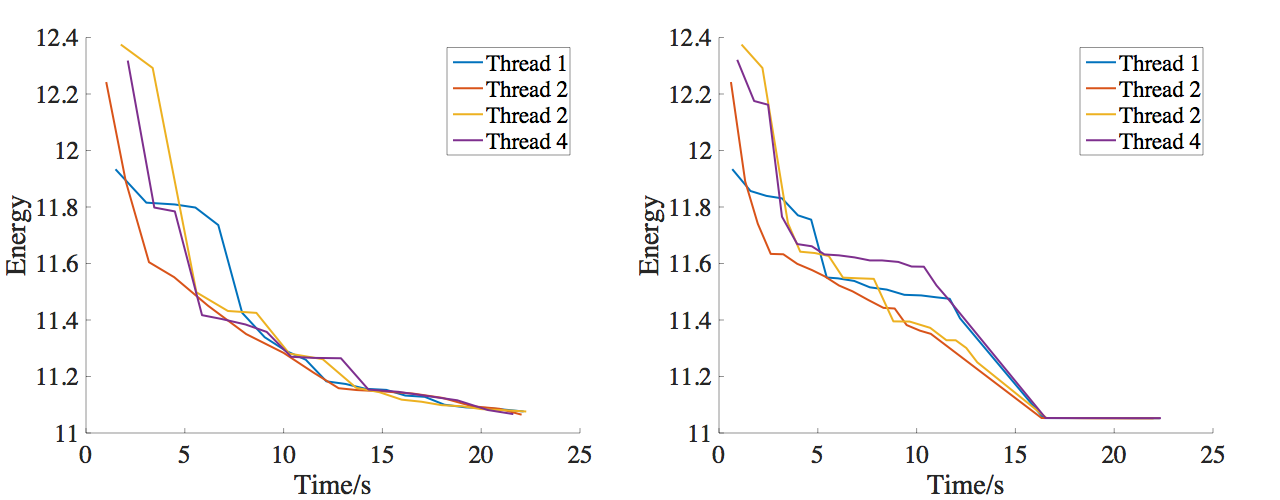
\includegraphics[width=\columnwidth]{figure/stereo_threads.png}
  \caption{Per thread energy. The left and right figures show the
    energy minimization process on each working thread of our method
    in SF-MF configuration and parallel $\alpha$-expansion method,
    respectively. The energy is in $\log$ scale}
  \label{fig:stereo_threads}
\end{figure}


Figure \ref{fig:stereo_global} shows the energy minimization process
against time. In this experiment, both PAE and SF-MF converge faster
than sequential method. However, since fusing solutions with multiple
labels by QPBO is slower than a single $\alpha$-expansion, PAE method
reaches convergence faster than SF-MF. Architectures with multiway
fusion, e.g. SF and SF-SS perform worse than PAE and SF-MF, because
the TRWS algorihtm used in multiway fusion is slower than multiple
$\alpha$-expansion. Finally, the line of hierarchy fusion only makes
jump when fusing on root node of the tree. This is because any fusion
step on non-root nodes only have partial label information.

Figure \ref{fig:stereo_threads} shows the per-thread energy
minimization process in SF-MF and PAE. The per-thread energy in SF-MF
architecture decreases more uniformly than that of PAE. In the
scenario where we need to query the best solution so far before the
whole optimization converges, SF-MF architecture is a better choice.

For a easy optimization problem as shown in this section, our full
architecture with solution sharing and multiway fusion actually makes
convergence slower by adopting sophisticated algorihtm and introducing
multi-threading overhead. However, we can easily configure the
architecture to make it better fit the problem, e.g. turn off multiway
fusion and/or solution sharing.

